\documentclass[12pt]{article}
\usepackage[margin=1in]{geometry}
\usepackage{amsmath}
\usepackage{amssymb}
\usepackage{enumitem}
\usepackage{xcolor}
\usepackage{tikz}
\usepackage{pgfplots}
\pgfplotsset{compat=1.17}
\usepackage{tcolorbox}
\usepackage{booktabs}

\definecolor{principleblue}{RGB}{0,102,204}
\definecolor{examplegreen}{RGB}{0,128,0}
\definecolor{warningred}{RGB}{204,0,0}

\newtcolorbox{keyidea}[1][]{
  colback=principleblue!5,
  colframe=principleblue,
  fonttitle=\bfseries,
  title=#1
}

\newtcolorbox{example}[1][]{
  colback=examplegreen!5,
  colframe=examplegreen,
  fonttitle=\bfseries,
  title=#1
}

\newtcolorbox{warning}[1][]{
  colback=warningred!5,
  colframe=warningred,
  fonttitle=\bfseries,
  title=#1
}

\title{\textbf{ECO310 Problem Set 3, Question 1 Teaching Guide} \\
\large Cost Functions \& Monopoly Pricing}
\author{Comprehensive Lecture Review}
\date{March 28, 2026}

\begin{document}

\maketitle

\tableofcontents
\newpage

\section{Overview: What You Need to Know}

This guide covers \textbf{two major topics} from Lectures 11 \& 12 that you missed:

\begin{enumerate}
\item \textbf{Question 1A}: Deriving cost functions from production technology
\item \textbf{Question 1B}: Monopoly profit maximization
\end{enumerate}

\begin{keyidea}[Big Picture]
We're transitioning from \textbf{consumer theory} (how consumers make choices) to \textbf{producer theory} (how firms make production decisions). This involves:
\begin{itemize}
\item Understanding how firms produce goods (production functions)
\item How much it costs to produce goods (cost functions)
\item How firms price their products (perfect competition vs. monopoly)
\end{itemize}
\end{keyidea}

\newpage

\section{Part 1: Production Functions and Cost Functions (Question 1A)}

\subsection{What is a Production Function?}

\begin{keyidea}[Production Function]
A \textbf{production function} shows the relationship between inputs (like labor, capital) and outputs (goods produced).

General form: $q = f(L, K)$ where:
\begin{itemize}
\item $q$ = quantity of output produced
\item $L$ = labor input (number of workers or hours)
\item $K$ = capital input (machines, equipment)
\end{itemize}
\end{keyidea}

\subsection{Common Production Functions You'll See}

\begin{enumerate}
\item \textbf{Linear}: $q = aL + bK$ (constant returns, each input adds constant amount)

\item \textbf{Square root}: $q = \sqrt{L}$ or $q = 1 + \sqrt{L}$ (\textbf{this is Question 1A!})

\item \textbf{Cobb-Douglas}: $q = L^\alpha K^\beta$ (most common in economics)

\item \textbf{Quadratic}: $q = L^2$ or $q = K^2$
\end{enumerate}

\subsection{From Production to Cost: The Key Steps}

\begin{keyidea}[Deriving Cost Functions: The Process]
To find how much it costs to produce $q$ units, follow these steps:

\textbf{Step 1}: Start with production function $q = f(L, K)$

\textbf{Step 2}: \textbf{Invert} to get input in terms of output
\begin{itemize}
\item Solve for $L$ or $K$ as a function of $q$
\item Example: If $q = \sqrt{L}$, then $L = q^2$
\end{itemize}

\textbf{Step 3}: Multiply by input prices
\begin{itemize}
\item If labor costs $w$ per unit: $\text{Cost} = w \cdot L$
\item If capital costs $r$ per unit: $\text{Cost} = r \cdot K$
\item Total cost: $C(q) = wL(q) + rK(q)$
\end{itemize}

\textbf{Step 4}: Identify fixed vs. variable costs
\begin{itemize}
\item Fixed costs ($F$): Don't change with $q$ (rent, overhead)
\item Variable costs ($VC(q)$): Change with $q$ (labor, materials)
\item $C(q) = F + VC(q)$
\end{itemize}
\end{keyidea}

\newpage

\subsection{Worked Example: Similar to Question 1A}

\begin{example}[Deriving a Cost Function]
\textbf{Setup}: A firm has production function $q = \sqrt{L}$ where $L$ is labor. Each unit of labor costs $w = \$4$.

\textbf{Question}: Find the cost function $C(q)$.

\vspace{0.3cm}
\textbf{Solution}:

\textbf{Step 1}: Production function is $q = \sqrt{L}$

\textbf{Step 2}: Invert to get $L$ in terms of $q$:
\begin{align*}
q &= \sqrt{L} \\
q^2 &= L \quad \text{(square both sides)}
\end{align*}

So we need $L = q^2$ units of labor to produce $q$ units of output.

\textbf{Step 3}: Multiply by wage rate:
\begin{align*}
C(q) &= w \cdot L \\
&= 4 \cdot q^2 \\
&= 4q^2
\end{align*}

\textbf{Answer}: $C(q) = 4q^2$

\vspace{0.3cm}
\textbf{Interpretation}: To produce 1 unit costs $\$4$. To produce 2 units costs $\$16$. To produce 3 units costs $\$36$. Costs increase \textit{quadratically} with output!
\end{example}

\subsection{Important Cost Function Terminology}

Once you have $C(q)$, you can derive several important concepts:

\begin{keyidea}[Cost Function Components]
\begin{enumerate}
\item \textbf{Total Cost}: $C(q) = F + VC(q)$
\begin{itemize}
\item $F$ = fixed costs (constant, independent of $q$)
\item $VC(q)$ = variable costs (depends on $q$)
\end{itemize}

\item \textbf{Marginal Cost}: $MC(q) = C'(q) = \frac{dC}{dq}$
\begin{itemize}
\item Cost of producing one more unit
\item \textbf{Key for profit maximization!}
\end{itemize}

\item \textbf{Average Cost}: $AC(q) = \frac{C(q)}{q}$
\begin{itemize}
\item Cost per unit
\end{itemize}

\item \textbf{Average Variable Cost}: $AVC(q) = \frac{VC(q)}{q}$
\begin{itemize}
\item Variable cost per unit
\item Important for shutdown decisions (firms shut down if $p < \min AVC$)
\end{itemize}
\end{enumerate}
\end{keyidea}

\newpage

\subsection{Question 1A: Step-by-Step Approach}

Now let's apply this to your actual problem:

\begin{tcolorbox}[colback=yellow!10, colframe=orange, title=\textbf{Problem 1A}]
A firm produces output according to $q = 1 + \sqrt{L}$ where $q$ is output and $L$ is labor. Each labor unit costs $\$2$. Find the cost function $C(q)$.
\end{tcolorbox}

\vspace{0.3cm}

\textbf{Your Turn - Follow These Steps}:

\textbf{Step 1}: Write down the production function
\begin{align*}
q = 1 + \sqrt{L}
\end{align*}

\textbf{Step 2}: Solve for $L$ in terms of $q$ (invert the function)
\begin{align*}
q &= 1 + \sqrt{L} \\
q - 1 &= \sqrt{L} \quad \text{(subtract 1 from both sides)} \\
(q-1)^2 &= L \quad \text{(square both sides)}
\end{align*}

So $L(q) = (q-1)^2$

\textbf{Step 3}: Multiply by wage rate ($w = 2$)
\begin{align*}
C(q) &= w \cdot L(q) \\
&= 2 \cdot (q-1)^2 \\
&= 2(q^2 - 2q + 1) \\
&= 2q^2 - 4q + 2
\end{align*}

\begin{keyidea}[Answer to 1A]
$$\boxed{C(q) = 2q^2 - 4q + 2 \quad \text{or equivalently} \quad C(q) = 2(q-1)^2}$$

\textbf{Components}:
\begin{itemize}
\item Fixed cost: $F = 2$ (the constant term when $q = 0$, though technically $C(0) = 2$)
\item Variable cost: $VC(q) = 2q^2 - 4q$ (the part that depends on $q$)
\item Marginal cost: $MC(q) = C'(q) = 4q - 4 = 4(q-1)$
\end{itemize}
\end{keyidea}

\begin{warning}[Common Mistake]
Don't forget to square \textbf{both terms} when you have $(q-1)^2$:
\begin{align*}
(q-1)^2 = q^2 - 2q + 1 \quad \text{\checkmark Correct}
\end{align*}
NOT just $q^2 - 1$ or $q^2 + 1$!
\end{warning}

\newpage

\section{Part 2: Monopoly and Profit Maximization (Question 1B)}

\subsection{Perfect Competition vs. Monopoly: The Big Difference}

\begin{keyidea}[Market Structures]
\begin{center}
\begin{tabular}{p{3cm}|p{5cm}|p{5cm}}
\toprule
\textbf{Feature} & \textbf{Perfect Competition} & \textbf{Monopoly} \\
\midrule
Number of firms & Many small firms & One firm (the monopolist) \\
\midrule
Price-taking? & Yes - firms take price as given & No - firm sets price \\
\midrule
Demand curve & Horizontal (perfectly elastic) at market price $p$ & Downward-sloping market demand $P^D(Q)$ \\
\midrule
Marginal Revenue & $MR = p$ (constant) & $MR = P^D(Q) + Q \cdot \frac{dP^D}{dQ}$ (decreasing) \\
\midrule
Profit max & $p = MC$ & $MR = MC$ \\
\bottomrule
\end{tabular}
\end{center}
\end{keyidea}

\subsection{Why Does Market Structure Matter?}

\textbf{Perfect Competition}: Imagine you're selling pencils at a farmer's market. There are 100 other vendors selling identical pencils.
\begin{itemize}
\item If everyone sells at $\$1$, you must also sell at $\$1$
\item If you charge $\$1.10$, nobody buys from you
\item You're a \textbf{price-taker} - you take the market price as given
\item Your revenue from selling $q$ units: $R(q) = p \cdot q = 1 \cdot q$
\item Marginal revenue: $MR = \frac{dR}{dq} = 1$ (constant!)
\end{itemize}

\textbf{Monopoly}: Now imagine you're Apple in 2010, the only company selling tablets.
\begin{itemize}
\item You control the entire market
\item If you want to sell more units, you must \textbf{lower the price}
\item The market demand curve tells you: at price $P$, consumers want $Q^D(P)$ units
\item You must decide: high price + low quantity, or low price + high quantity?
\item Your revenue: $R(Q) = P^D(Q) \cdot Q$ (price depends on quantity!)
\end{itemize}

\newpage

\subsection{Understanding Demand Curves}

\begin{keyidea}[Demand vs. Inverse Demand]
Two ways to express the same relationship:

\textbf{Demand curve}: $Q^D(P)$ tells you quantity demanded at price $P$
\begin{itemize}
\item Example: $Q^D(P) = 200 - 5P$
\item "At price $P = 10$, consumers demand $Q = 200 - 50 = 150$ units"
\end{itemize}

\textbf{Inverse demand curve}: $P^D(Q)$ tells you the price at which you can sell $Q$ units
\begin{itemize}
\item Solve for $P$: $Q = 200 - 5P \implies 5P = 200 - Q \implies P = 40 - \frac{Q}{5}$
\item Example: $P^D(Q) = 40 - \frac{Q}{5}$
\item "To sell $Q = 150$ units, you must charge price $P = 40 - 30 = 10$"
\end{itemize}

\textbf{For monopoly problems, we typically use inverse demand} $P^D(Q)$ because the monopolist chooses quantity $Q$ and the price is determined by the demand curve.
\end{keyidea}

\subsection{Monopolist's Revenue and Marginal Revenue}

\begin{keyidea}[Monopolist's Revenue]
\textbf{Total Revenue}:
\begin{align*}
R(Q) = P^D(Q) \cdot Q
\end{align*}

The monopolist sells $Q$ units at price $P^D(Q)$.

\vspace{0.3cm}

\textbf{Marginal Revenue}: Revenue from selling one more unit
\begin{align*}
MR(Q) = \frac{dR}{dQ} = \frac{d}{dQ}[P^D(Q) \cdot Q]
\end{align*}

Using the product rule:
\begin{align*}
MR(Q) = P^D(Q) + Q \cdot \frac{dP^D}{dQ}
\end{align*}

Since demand is downward-sloping, $\frac{dP^D}{dQ} < 0$, so:
$$\boxed{MR(Q) < P^D(Q) \text{ for a monopolist}}$$
\end{keyidea}

\begin{warning}[Critical Insight]
\textbf{Why is $MR < P$ for a monopolist?}

When a monopolist sells one more unit:
\begin{enumerate}
\item \textbf{Gain}: Revenue from selling that unit at price $P$ ($+P$)
\item \textbf{Loss}: To sell more, price must drop, reducing revenue on \textit{all previous units} ($-Q \cdot \Delta P$)
\end{enumerate}

Example: If you sell 100 tablets at $\$500$ each ($R = \$50,000$), and to sell 101 tablets you must drop price to $\$499$:
\begin{itemize}
\item Gain from 101st tablet: $+\$499$
\item Loss on first 100 tablets: $-100 \times \$1 = -\$100$
\item Net marginal revenue: $\$499 - \$100 = \$399 < \$499$ (the price!)
\end{itemize}
\end{warning}

\newpage

\subsection{Monopoly Profit Maximization}

\begin{keyidea}[Monopolist's Problem]
The monopolist wants to maximize profit:
\begin{align*}
\Pi(Q) = R(Q) - C(Q) = P^D(Q) \cdot Q - C(Q)
\end{align*}

\textbf{First Order Condition}:
\begin{align*}
\frac{d\Pi}{dQ} = 0 \implies MR(Q) = MC(Q)
\end{align*}

\textbf{Steps to solve}:
\begin{enumerate}
\item Write out profit function: $\Pi(Q) = P^D(Q) \cdot Q - C(Q)$
\item Take derivative with respect to $Q$: $\frac{d\Pi}{dQ} = MR - MC$
\item Set equal to zero: $MR = MC$
\item Solve for optimal quantity $Q^*$
\item Plug $Q^*$ into inverse demand to find price: $P^* = P^D(Q^*)$
\end{enumerate}
\end{keyidea}

\subsection{Calculating Marginal Revenue: The Formula}

\begin{keyidea}[MR Formula for Linear Demand]
If inverse demand is \textbf{linear}: $P^D(Q) = a - bQ$

Then marginal revenue is: $MR(Q) = a - 2bQ$

\textbf{Rule of thumb}: MR has the \textbf{same intercept} but \textbf{twice the slope} of inverse demand!

\vspace{0.3cm}
\textbf{Why?}
\begin{align*}
R(Q) &= P^D(Q) \cdot Q = (a - bQ) \cdot Q = aQ - bQ^2 \\
MR(Q) &= \frac{dR}{dQ} = a - 2bQ
\end{align*}
\end{keyidea}

\begin{example}[Computing MR]
\textbf{Inverse demand}: $P^D(Q) = 200 - 5Q$

\textbf{Marginal revenue}:
\begin{align*}
R(Q) &= P^D(Q) \cdot Q = (200 - 5Q) \cdot Q = 200Q - 5Q^2 \\
MR(Q) &= \frac{dR}{dQ} = 200 - 10Q
\end{align*}

Or use the shortcut: $P = 200 - 5Q \implies MR = 200 - 10Q$ (same intercept, double the slope!)
\end{example}

\newpage

\subsection{Worked Example: Monopoly Profit Maximization}

\begin{example}[Full Monopoly Problem]
\textbf{Setup}: A monopolist has cost function $C(Q) = Q^2 + 1$ and faces inverse demand $P^D(Q) = 400 - Q$.

\textbf{Question}: Find the profit-maximizing quantity and price.

\vspace{0.3cm}
\textbf{Solution}:

\textbf{Step 1}: Write profit function
\begin{align*}
\Pi(Q) &= R(Q) - C(Q) \\
&= P^D(Q) \cdot Q - C(Q) \\
&= (400 - Q) \cdot Q - (Q^2 + 1) \\
&= 400Q - Q^2 - Q^2 - 1 \\
&= 400Q - 2Q^2 - 1
\end{align*}

\textbf{Step 2}: Find marginal revenue and marginal cost
\begin{align*}
MR(Q) &= \frac{dR}{dQ} = \frac{d}{dQ}[(400-Q) \cdot Q] = 400 - 2Q \\
MC(Q) &= \frac{dC}{dQ} = 2Q
\end{align*}

\textbf{Step 3}: Set $MR = MC$
\begin{align*}
400 - 2Q &= 2Q \\
400 &= 4Q \\
Q^* &= 100
\end{align*}

\textbf{Step 4}: Find price by plugging into demand
\begin{align*}
P^* = P^D(Q^*) = 400 - 100 = 300
\end{align*}

\textbf{Answer}: The monopolist sells $Q^* = 100$ units at price $P^* = \$300$.

\vspace{0.3cm}
\textbf{Profit check}:
\begin{align*}
\Pi(100) &= 300 \cdot 100 - (100^2 + 1) \\
&= 30,000 - 10,001 \\
&= 19,999
\end{align*}

The monopolist makes $\$19,999$ in profit!
\end{example}

\newpage

\subsection{Question 1B: Step-by-Step Approach}

Now let's apply this to your actual problem:

\begin{tcolorbox}[colback=yellow!10, colframe=orange, title=\textbf{Problem 1B}]
Suppose the firm is a monopolist and faces demand curve $Q^D(P) = 200 - 5P$. The cost function is $C(q) = 2(q-1)^2$ from part (a). How much will the monopolist sell, and at what price?
\end{tcolorbox}

\vspace{0.3cm}

\textbf{Your Turn - Follow These Steps}:

\textbf{Step 1}: Convert demand to inverse demand
\begin{align*}
Q^D(P) &= 200 - 5P \\
5P &= 200 - Q \\
P^D(Q) &= 40 - \frac{Q}{5}
\end{align*}

\textbf{Step 2}: Write profit function
\begin{align*}
\Pi(Q) &= P^D(Q) \cdot Q - C(Q) \\
&= \left(40 - \frac{Q}{5}\right) \cdot Q - 2(Q-1)^2 \\
&= 40Q - \frac{Q^2}{5} - 2(Q^2 - 2Q + 1) \\
&= 40Q - \frac{Q^2}{5} - 2Q^2 + 4Q - 2 \\
&= 44Q - \frac{Q^2}{5} - 2Q^2 - 2
\end{align*}

Simplify the $Q^2$ terms:
\begin{align*}
-\frac{Q^2}{5} - 2Q^2 = -\frac{Q^2}{5} - \frac{10Q^2}{5} = -\frac{11Q^2}{5}
\end{align*}

So:
\begin{align*}
\Pi(Q) = 44Q - \frac{11Q^2}{5} - 2
\end{align*}

\textbf{Step 3}: Find MR and MC
\begin{align*}
MR(Q) &= \frac{d}{dQ}\left[\left(40 - \frac{Q}{5}\right) \cdot Q\right] = 40 - \frac{2Q}{5} \\
MC(Q) &= \frac{dC}{dQ} = \frac{d}{dQ}[2(Q-1)^2] = 2 \cdot 2(Q-1) = 4(Q-1) = 4Q - 4
\end{align*}

\newpage

\textbf{Step 4}: Set $MR = MC$
\begin{align*}
40 - \frac{2Q}{5} &= 4Q - 4 \\
40 + 4 &= 4Q + \frac{2Q}{5} \\
44 &= \frac{20Q}{5} + \frac{2Q}{5} \\
44 &= \frac{22Q}{5} \\
220 &= 22Q \\
Q^* &= 10
\end{align*}

\textbf{Step 5}: Find price
\begin{align*}
P^* = P^D(Q^*) = 40 - \frac{10}{5} = 40 - 2 = 38
\end{align*}

\begin{keyidea}[Answer to 1B]
$$\boxed{Q^* = 10 \text{ units, } P^* = \$38}$$

The monopolist will produce and sell 10 units at a price of $\$38$ per unit.

\vspace{0.3cm}
\textbf{Check}: Revenue = $38 \times 10 = \$380$

Cost = $C(10) = 2(10-1)^2 = 2(81) = \$162$

Profit = $380 - 162 = \$218$
\end{keyidea}

\newpage

\section{Additional Concepts: Full Context}

\subsection{Why Do We Care About Market Structure?}

\begin{keyidea}[Economic Efficiency]
\textbf{Perfect competition} leads to efficient outcomes:
\begin{itemize}
\item Price = Marginal cost ($P = MC$)
\item Consumer surplus + Producer surplus is maximized
\item No deadweight loss
\end{itemize}

\textbf{Monopoly} creates inefficiency:
\begin{itemize}
\item Price $>$ Marginal cost ($P > MC$)
\item Monopolist restricts quantity to raise price
\item Creates \textbf{deadweight loss} (lost welfare)
\item Transfers surplus from consumers to the monopolist
\end{itemize}
\end{keyidea}

\subsection{Graphical Intuition: Monopoly vs. Perfect Competition}

\begin{center}
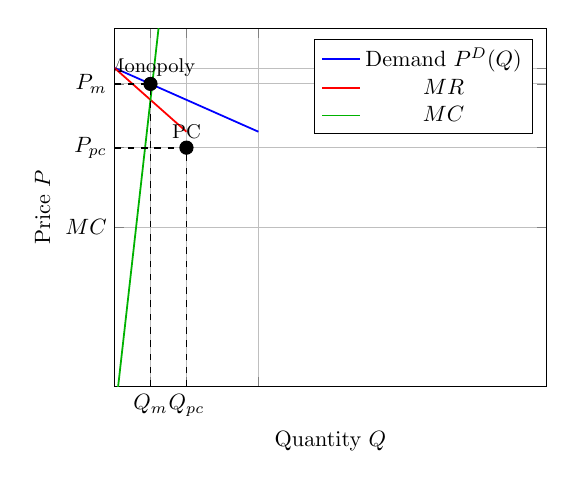
\begin{tikzpicture}[scale=0.8]
\begin{axis}[
    xlabel={Quantity $Q$},
    ylabel={Price $P$},
    xmin=0, xmax=120,
    ymin=0, ymax=45,
    xtick={10,20,40},
    xticklabels={$Q_m$,$Q_{pc}$},
    ytick={20,30,38,40},
    yticklabels={$MC$,$P_{pc}$,$P_m$},
    legend pos=north east,
    grid=major,
]

% Demand curve
\addplot[domain=0:40, samples=100, color=blue, thick] {40 - x/5};
\addlegendentry{Demand $P^D(Q)$}

% MR curve
\addplot[domain=0:20, samples=100, color=red, thick] {40 - 2*x/5};
\addlegendentry{$MR$}

% MC curve
\addplot[domain=0:40, samples=100, color=green!70!black, thick] {4*x - 4};
\addlegendentry{$MC$}

% Monopoly point
\addplot[only marks, mark=*, mark size=3pt, color=black] coordinates {(10,38)};
\node at (axis cs:10,40) {\small Monopoly};

% Perfect competition point
\addplot[only marks, mark=*, mark size=3pt, color=black] coordinates {(20,30)};
\node at (axis cs:20,32) {\small PC};

% Vertical lines
\addplot[dashed, thick] coordinates {(10,0) (10,38)};
\addplot[dashed, thick] coordinates {(20,0) (20,30)};

% Horizontal lines
\addplot[dashed, thick] coordinates {(0,38) (10,38)};
\addplot[dashed, thick] coordinates {(0,30) (20,30)};

\end{axis}
\end{tikzpicture}
\end{center}

\textbf{Key observations}:
\begin{enumerate}
\item Monopolist produces at $Q_m$ where $MR = MC$ (point at $Q=10$)
\item Perfect competition produces at $Q_{pc}$ where $P = MC$ (point at $Q=20$)
\item Monopolist restricts quantity ($Q_m < Q_{pc}$) and charges higher price ($P_m > P_{pc}$)
\item The area between is deadweight loss!
\end{enumerate}

\newpage

\subsection{Types of Costs: Complete Summary}

\begin{center}
\begin{tabular}{|p{3.5cm}|p{4cm}|p{6cm}|}
\hline
\textbf{Cost Type} & \textbf{Formula} & \textbf{Meaning} \\
\hline
\hline
Total Cost & $C(q) = F + VC(q)$ & Total cost of producing $q$ units \\
\hline
Fixed Cost & $F$ & Costs that don't change with output (rent, machines) \\
\hline
Variable Cost & $VC(q)$ & Costs that change with output (labor, materials) \\
\hline
Marginal Cost & $MC(q) = C'(q)$ & Cost of producing one more unit \\
\hline
Average Total Cost & $AC(q) = \frac{C(q)}{q}$ & Cost per unit \\
\hline
Average Variable Cost & $AVC(q) = \frac{VC(q)}{q}$ & Variable cost per unit \\
\hline
Average Fixed Cost & $AFC(q) = \frac{F}{q}$ & Fixed cost per unit (decreases as $q$ increases) \\
\hline
\end{tabular}
\end{center}

\subsection{Profit Maximization: All Market Structures}

\begin{keyidea}[Universal Profit Maximization Rule]
\textbf{All firms} (competitive or monopolist) maximize profit by producing where:
$$MR(Q) = MC(Q)$$

The difference is \textbf{what MR equals}:
\begin{itemize}
\item \textbf{Perfect competition}: $MR = P$ (constant)
\item \textbf{Monopoly}: $MR = P^D(Q) + Q \cdot \frac{dP^D}{dQ} < P$ (decreasing)
\end{itemize}
\end{keyidea}

\newpage

\section{Common Mistakes and How to Avoid Them}

\subsection{Mistake 1: Forgetting to Invert Production Function}

\begin{warning}[Don't Do This]
\textbf{Wrong}: $q = 1 + \sqrt{L} \implies C(q) = 2(1 + \sqrt{q})$

You can't just replace $L$ with $q$! You must \textbf{solve for $L$ first}.
\end{warning}

\textbf{Correct approach}:
\begin{align*}
q = 1 + \sqrt{L} \implies L = (q-1)^2 \implies C(q) = 2(q-1)^2
\end{align*}

\subsection{Mistake 2: Using Price Instead of MR for Monopolist}

\begin{warning}[Don't Do This]
\textbf{Wrong}: "Monopolist maximizes profit where $P = MC$"

This is the \textbf{perfect competition} rule! For monopolists, $MR \neq P$.
\end{warning}

\textbf{Correct approach}: Monopolist maximizes where $MR = MC$, where:
\begin{align*}
MR = P^D(Q) + Q \cdot \frac{dP^D}{dQ} < P^D(Q)
\end{align*}

\subsection{Mistake 3: Confusing Demand and Inverse Demand}

\begin{warning}[Don't Do This]
Given $Q^D(P) = 200 - 5P$:

\textbf{Wrong}: "Revenue = $(200 - 5P) \cdot P$"

This mixes up the variable! If you're using $Q$ as your choice variable (which monopolists do), you need inverse demand.
\end{warning}

\textbf{Correct approach}:
\begin{enumerate}
\item Convert to inverse demand: $P^D(Q) = 40 - \frac{Q}{5}$
\item Revenue: $R(Q) = P^D(Q) \cdot Q = \left(40 - \frac{Q}{5}\right) \cdot Q$
\end{enumerate}

\subsection{Mistake 4: Not Simplifying Before Taking Derivatives}

\begin{warning}[Don't Do This]
\textbf{Wrong}: Taking derivative of $\Pi(Q) = (40 - \frac{Q}{5}) \cdot Q - 2(Q-1)^2$ directly without expanding.

This leads to messy product rule and chain rule applications.
\end{warning}

\textbf{Correct approach}: Expand everything first:
\begin{align*}
\Pi(Q) &= 40Q - \frac{Q^2}{5} - 2Q^2 + 4Q - 2 \\
&= 44Q - \frac{11Q^2}{5} - 2
\end{align*}

Now taking the derivative is easy!

\newpage

\section{Practice Problems}

\subsection{Practice Problem 1: Cost Functions}

\textbf{Problem}: A firm has production function $q = 2\sqrt{L}$ where labor costs $\$9$ per unit. Find $C(q)$.

\vspace{3cm}

\subsection{Practice Problem 2: Monopoly}

\textbf{Problem}: A monopolist has $C(Q) = 3Q^2$ and faces demand $Q^D(P) = 100 - 2P$. Find optimal $Q$ and $P$.

\vspace{5cm}

\subsection{Practice Problem 3: Comparing Outcomes}

\textbf{Problem}: Using the same demand and cost as Practice Problem 2, what would $Q$ and $P$ be under perfect competition?

\vspace{3cm}

\newpage

\section{Solutions to Practice Problems}

\subsection{Solution 1}

\textbf{Given}: $q = 2\sqrt{L}$, $w = 9$

\textbf{Step 1}: Invert production function
\begin{align*}
q &= 2\sqrt{L} \\
\frac{q}{2} &= \sqrt{L} \\
\left(\frac{q}{2}\right)^2 &= L \\
L &= \frac{q^2}{4}
\end{align*}

\textbf{Step 2}: Multiply by wage
\begin{align*}
C(q) = 9 \cdot \frac{q^2}{4} = \frac{9q^2}{4}
\end{align*}

\textbf{Answer}: $C(q) = \frac{9q^2}{4}$

\subsection{Solution 2}

\textbf{Given}: $C(Q) = 3Q^2$, $Q^D(P) = 100 - 2P$

\textbf{Step 1}: Inverse demand
\begin{align*}
Q = 100 - 2P \implies P^D(Q) = 50 - \frac{Q}{2}
\end{align*}

\textbf{Step 2}: Find MR and MC
\begin{align*}
MR &= 50 - Q \quad \text{(double the slope)} \\
MC &= 6Q
\end{align*}

\textbf{Step 3}: Set $MR = MC$
\begin{align*}
50 - Q &= 6Q \\
50 &= 7Q \\
Q^* &= \frac{50}{7} \approx 7.14
\end{align*}

\textbf{Step 4}: Find price
\begin{align*}
P^* = 50 - \frac{50/7}{2} = 50 - \frac{25}{7} = \frac{325}{7} \approx 46.43
\end{align*}

\textbf{Answer}: $Q^* = \frac{50}{7} \approx 7.14$ units, $P^* \approx \$46.43$

\subsection{Solution 3}

\textbf{Perfect competition}: Set $P = MC$

\begin{align*}
P &= 50 - \frac{Q}{2} \quad \text{(from inverse demand)} \\
MC &= 6Q \\
50 - \frac{Q}{2} &= 6Q \\
50 &= 6Q + \frac{Q}{2} = \frac{13Q}{2} \\
Q_{pc} &= \frac{100}{13} \approx 7.69 \\
P_{pc} &= 6 \cdot \frac{100}{13} = \frac{600}{13} \approx 46.15
\end{align*}

\textbf{Comparison}:
\begin{itemize}
\item Monopoly: $Q = 7.14$, $P = 46.43$
\item Perfect competition: $Q = 7.69$, $P = 46.15$
\item Monopolist produces less and charges more!
\end{itemize}

\newpage

\section{Quick Reference: Formulas You Need}

\begin{tcolorbox}[colback=blue!5, colframe=blue!50!black, title=\textbf{Essential Formulas Cheat Sheet}]

\textbf{Cost Functions}:
\begin{itemize}
\item $C(q) = F + VC(q)$ (total = fixed + variable)
\item $MC(q) = C'(q)$ (marginal cost)
\item $AC(q) = \frac{C(q)}{q}$ (average cost)
\end{itemize}

\vspace{0.3cm}

\textbf{Revenue}:
\begin{itemize}
\item $R(Q) = P \cdot Q$ (revenue = price $\times$ quantity)
\item For monopolist: $R(Q) = P^D(Q) \cdot Q$ (price depends on $Q$!)
\end{itemize}

\vspace{0.3cm}

\textbf{Marginal Revenue}:
\begin{itemize}
\item Perfect competition: $MR = P$ (constant)
\item Monopoly: $MR = P^D(Q) + Q \cdot \frac{dP^D}{dQ}$
\item For linear demand $P = a - bQ$: $MR = a - 2bQ$
\end{itemize}

\vspace{0.3cm}

\textbf{Profit}:
\begin{itemize}
\item $\Pi(Q) = R(Q) - C(Q)$
\item Maximize: $\frac{d\Pi}{dQ} = 0 \implies MR = MC$
\end{itemize}

\vspace{0.3cm}

\textbf{Inverse Demand}:
\begin{itemize}
\item Given $Q^D(P) = a - bP$, inverse is $P^D(Q) = \frac{a}{b} - \frac{Q}{b}$
\item Example: $Q = 200 - 5P \implies P = 40 - \frac{Q}{5}$
\end{itemize}

\end{tcolorbox}

\section{Final Checklist for Problem Set 3, Question 1}

\begin{enumerate}[label=\protect\checkmark]
\item \textbf{Question 1A}:
\begin{itemize}
\item Invert production function $q = 1 + \sqrt{L}$ to get $L = (q-1)^2$
\item Multiply by wage: $C(q) = 2(q-1)^2 = 2q^2 - 4q + 2$
\item Check by verifying $MC = C'(q) = 4q - 4$
\end{itemize}

\item \textbf{Question 1B}:
\begin{itemize}
\item Convert demand to inverse: $P^D(Q) = 40 - \frac{Q}{5}$
\item Find MR: $MR = 40 - \frac{2Q}{5}$
\item Find MC from part (a): $MC = 4Q - 4$
\item Set $MR = MC$ and solve: $Q^* = 10$
\item Find price: $P^* = 40 - 2 = 38$
\end{itemize}
\end{enumerate}

\vspace{1cm}

\begin{center}
\textbf{\Large You're ready to solve the problem!}

Good luck, and remember: take it step by step!
\end{center}

\end{document}
